%#MAKEINDEX makeindex interim01
\documentclass[10pt,a4j]{ujarticle}

\input{include/macro.tex}
\input{include/preamble.tex}

\begin{document}
%%%%%%%%%%%%%%%%%%%%%%%%%%%%%%%%%%%%%%%%%%%%%%%%%%%%%%%%%%%%%%%%%%%%%%
\section{物品一覧}
今回の配布品,引継ぎ品,購入品についてそれぞれ,以降の表にまとめる.ただし,購入品について※印がついた部品は,購入してテストした結果,使用しなかったものである.\\

今回ロボットにかかった合計金額は, $\yen 76,786$である.

\begin{table}[h]
	\centering
	\caption{配布品一覧}
	\includegraphics[clip,scale=0.4]{haihu.eps}
    \label{haihu}
\end{table}

\begin{table}[h]
	\centering
	\caption{引継ぎ品一覧}
	\includegraphics[clip,scale=0.4]{hikitsugi.eps}
 \label{hikitsugi}
\end{table}

\begin{table}[h]
	\centering
	\caption{購入品一覧}
	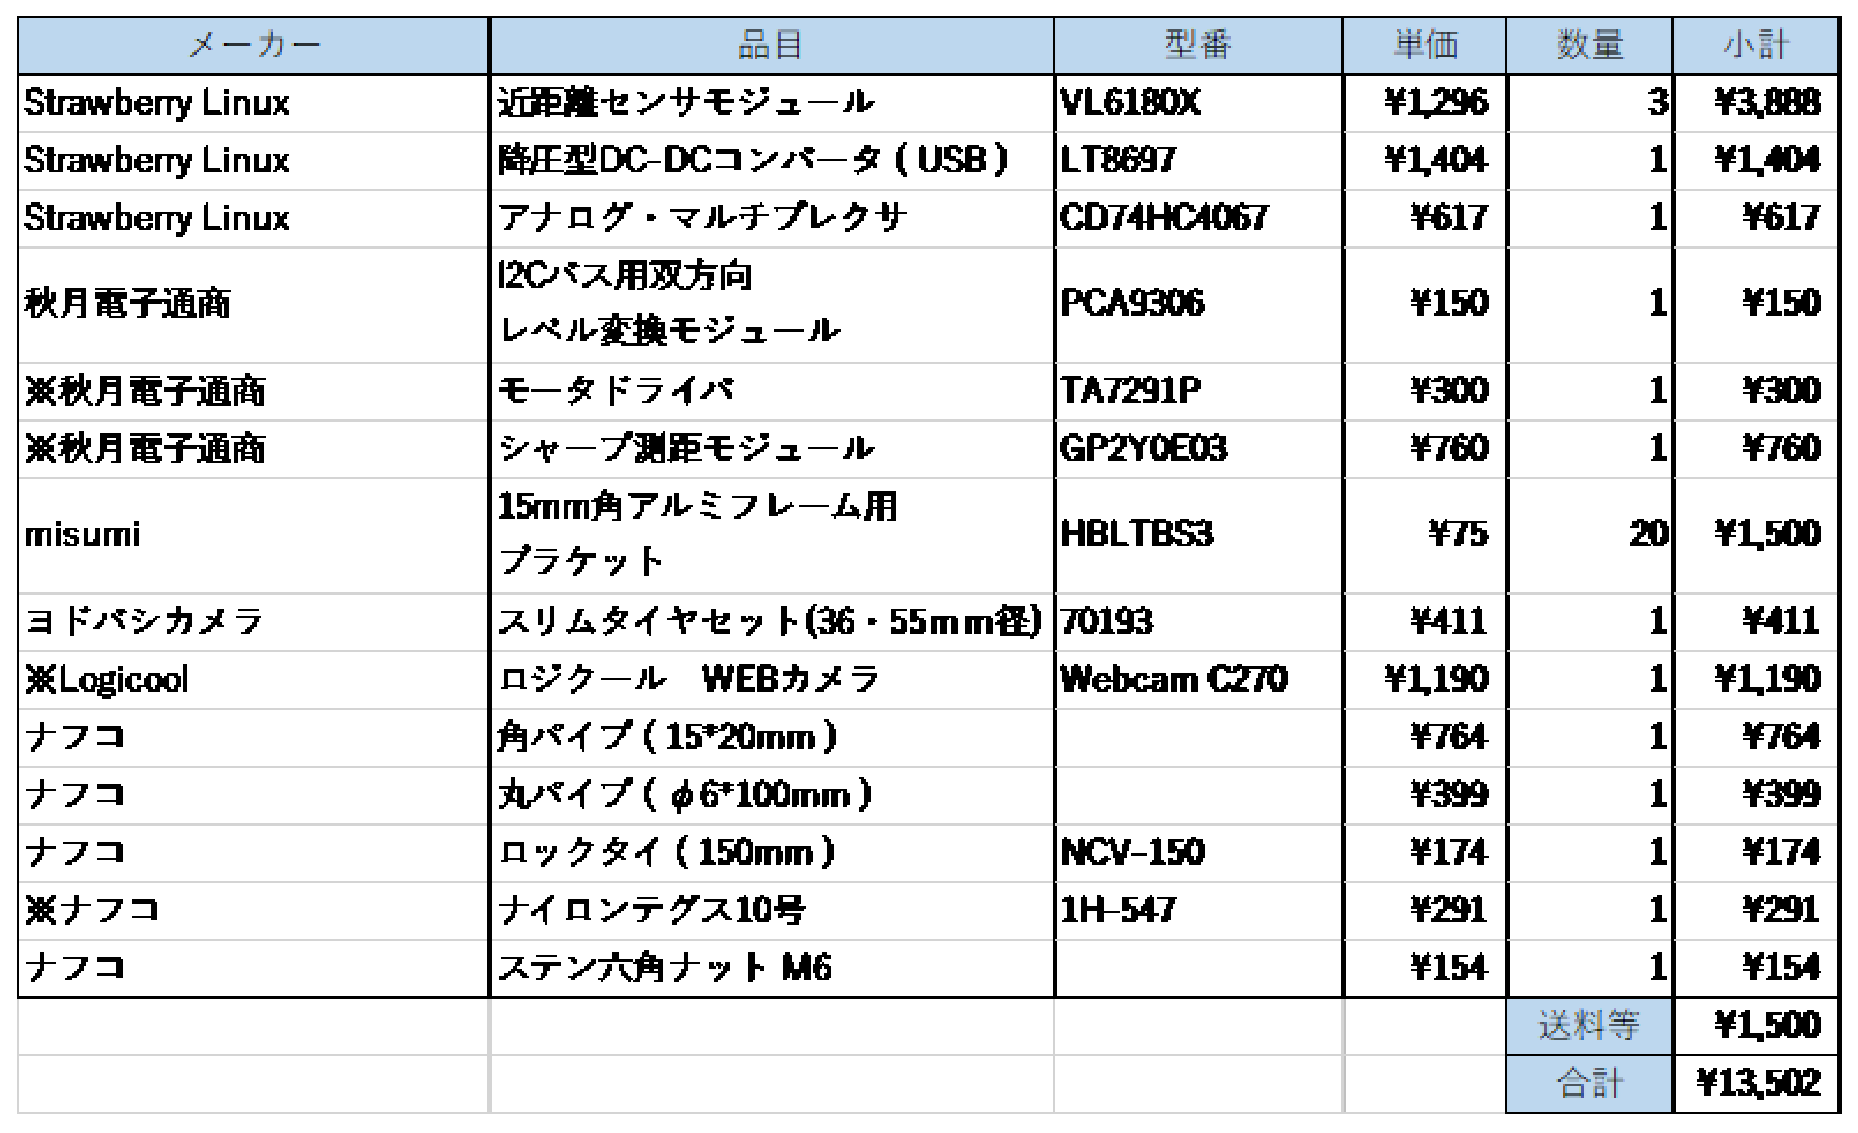
\includegraphics[clip,scale=0.4]{kokunyu.eps}
    \label{kounyu}
\end{table}
%%%%%%%%%%%%%%%%%%%%%%%%%%%%%%%%%%%%%%%%%%%%%%%%%%%%%%%%%%%%%%%%%%%%%%%%%%%%
\end{document}